\section{Review of physics-based EM modelling and analysis methods}
\label{sec:reliability_modeling}

EM is a physical phenomenon of the migration of metal atoms along a
direction of the applied electrical field. This oriented atomic flow,
which is caused mostly by the momentum exchange between atoms and the
conducting electrons, results in metal density depletion at the
cathode, and a corresponding metal accumulation at the anode end of
the metal wire. Due to the passivation of copper wires from the dual
damascene copper interconnect technology, hydrostatic stress will
build up from the metal concentration changes at those nodes, which
will lead to void nucleation when the stress reach to the critical
stress and following up failures of the wires as results of the void
growth.

EM phenomena and EM modeling have been intensively studied and some
important physics-based EM models have been proposed in the past two
decades~\cite{deOrio:2010}. Korhonen proposed the important EM model
to describe the EM-induced stress evolution of passivated interconnect
wires and its analytic solution for a simple wire structure in
1993~\cite{Korhonen:jap1993}, which was further developed by many
researchers~\cite{Clement:1999tcad, Sukharev:2015jap}. Specifically,
for a confined/passivated metal line, the hydrostatic stress
distribution $\sigma(x,t)$ along the metal wire can be described by a
one-dimensional diffusion-like equation, given
by:~\cite{Korhonen:jap1993}
% \begin{equation}
% \label{eq:basic_em}
% \frac{\partial \sigma(x,t)}{\partial t}=\frac{\partial }{\partial x}\left[\frac{D_aB\Omega}{kT}\left(\frac{\partial \sigma(x,t)}{\partial x}+\frac{Z^*e\rho}{\Omega}j\right)\right]
% \end{equation}
% where $\sigma$ is the hydrostatic stress, $t$ is the time, $D_a$ is
% the atomic diffusivity, $B$ is the effective bulk modulus, $\Omega$ is
% the atomic volume, $k$ is the Boltzman's constant, $T$ is the absolute
% temperature, $Z^*$ is the effective charge number, $e$ is the electron
% charge, $\rho$ is the resistivity, and $j$ is the current density.
%
% The advantage of this model is that the evolution of hydrostatic
% stress in a confined line can be calculated in a closed-form
% expression, which has been widely used in EM analysis.

% It should be noted that the closed-form expression reported in
% \cite{Korhonen:jap1993} is only applicable to a single wire case while
% it can not be used to calculate the hydrostatic stress during EM for
% multi-segment interconnect wires. In this paper, we extend the
% Korhonen equation \eqref{eq:basic_em} to allow for a general
% multi-segment interconnect wire.
%
% For the convenience of following
% description, we rewrite the Korhonen equation \eqref{eq:basic_em} as a
% compact form:
\begin{equation}
\label{eq:basic_em_s}
\frac{\partial \sigma(x,t)}{\partial t}=\frac{\partial }{\partial x}\left[\kappa\left(\frac{\partial \sigma(x,t)}{\partial x}+G\right)\right]
\end{equation}
where $\kappa=\frac{D_aB\Omega}{kT}$ is the stress diffusivity
affected by temperature $T$ and $G=\frac{Z^*e\rho}{\Omega}j$ is the EM
driving force. Moreover, $D_a=D_0e^{-\frac{E_a}{kT}}$ is the effective
atomic diffusion coefficient. $D_0$ and $E_a$ stand for the
pre-exponential factor and the activation energy, respectively. The
Korhonen equation \eqref{eq:basic_em_s} has different analytical
solutions with different boundary conditions (BCs). Following the idea
in \cite{Korhonen:jap1993}, we assume that the stress diffusivity
$\kappa$ does not depend on time. During the void nucleation phase of
EM, the atom fluxes are blocked at both wire ends $x=0$ and $x=L$ at
any moment in time. The initial stress value during the void
nucleation phase is set to be zero. Thus, the closed-form solution of
the stress evolution equation for a single segment wire can be given
as follows \cite{Korhonen:jap1993}:
\begin{equation} \label{eq:korhonen_sol}
\begin{split}
\sigma(x,t)&= \sigma_T+ GL\{\frac{1}{2}-\frac{x}{L}\\
&-4\sum\limits_{n=0}^{\infty}\frac{\cos((2n+1)\pi
\frac{x}{L})}{(2n+1)^2\pi^2\exp((2n+1)^2\pi^2\frac{\kappa
t}{L^2})}\}.
\end{split}
\end{equation}
where $\sigma_T$ is the pre-existing residual stress due to a thermal
process. If we only keep the slowest decaying term of the infinite
series in \eqref{eq:korhonen_sol}, we can compute the time to
nucleation. This happens when the wire stress $\sigma(x,t)$ has
reached a critical stress $\sigma_{crit}$, then the void
nucleation time $t_{nuc}$ can be obtained by solving the equation
$\sigma(x,t_{nuc})=\sigma_{crit}$~\cite{HuangYu:DAC'14}.

The physics-based EM model proposed
in~\cite{HuangYu:DAC'14,HuangTan:TCAD'16} was extended further to deal
with multi-branch interconnects, in which the projected steady-state
EM-induced stress of each branch without considering other branches is
first computed. Then the branch stresses are used to compute the total
stress distributions in a tree for calculating the final time to
failure if some of the stress is larger than the critical stress. The
drawback of this work is that it totally ignores all the dynamic
evolutions of stress over time and the interactions of void nucleation
process among branches. As a result, it still can't provide analytic
expression for the time-dependent hydrostatic evolution of hydrostatic
stress to determine the failures for multi-branch interconnect wires.

Recently, a voltage-based EM modeling and immortality check technique
for general interconnect tree structures has been
proposed~\cite{SunDemircan:ICCAD'16}. In this work, the steady-state
hydrostatic stress continuous equations are formed first and the
steady state stress at every node of the tree are then computed in
terms of node voltages and wire layout parameters. By checking the
largest stress over all the tree nodes, one can ensure that the tree
never fails if the largest stress is less than the critical stress. It
is very help for fast EM immortality check. But, this method still
can't give the time when the wire is predicted to fail. Following a
different direction, a research effort was carried out recently to
develop time-dependent stress evolution analytic solution for
multi-branch interconnect
tree~\cite{ChenHuang:DAC'15,ChenTan:TCAD'16}.  In this approach,
analytic solutions by means of the Laplace transformation method for
stress evolution were derived for three specific interconnect
structures: the straight-line 3-terminal wires, the T-shape 4-terminal
wires and the cross-shape 5-terminal wires. It was also shown that a
few dominant terms can be used for sufficiently accurate
solution. But, the proposed solution is not still general enough for
multi-segment interconnect wires shown in Fig.~\ref{fig:4seg-demo}.



% \begin{figure}[ht] \centering \subfigure[]{
%     \vspace{-0.2in}
%     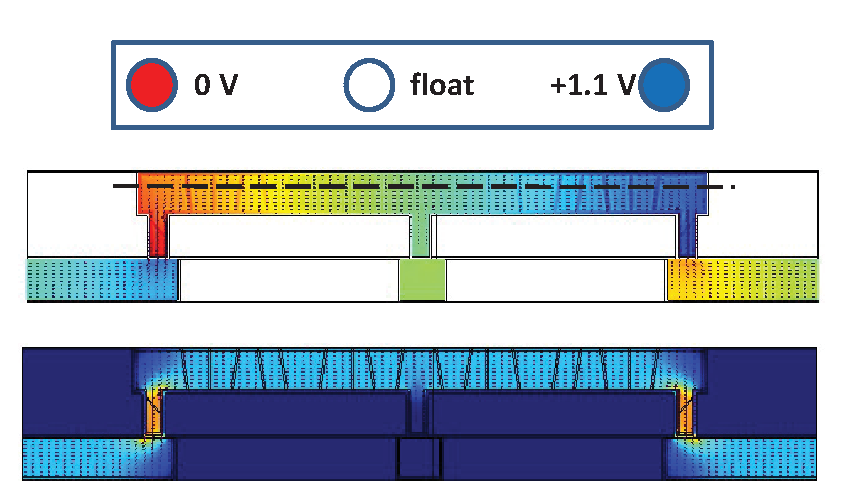
\includegraphics[width=44mm]{3_terminal_model.eps}
%     \label{fig:3_terminal_model}}
%     \subfigure[]{
%     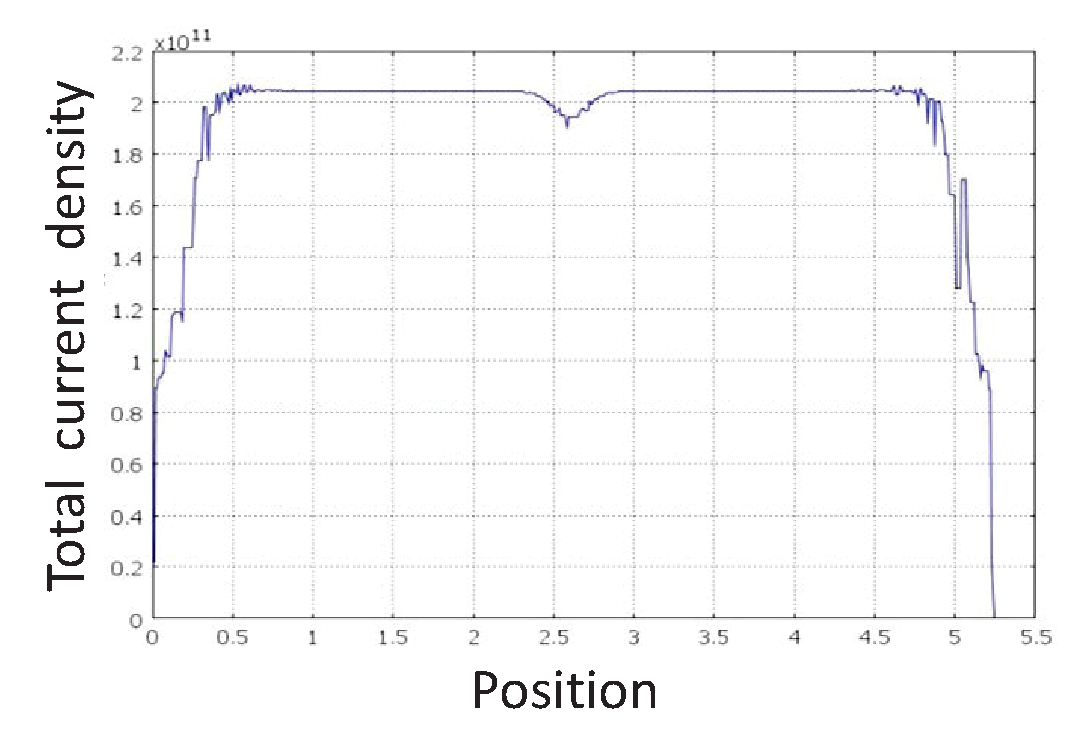
\includegraphics[width=37mm]{3_terminal_current.eps}
%     \label{fig:3_terminal_current}}
%     \vspace{-0.12in}
%         \subfigure[]{
%     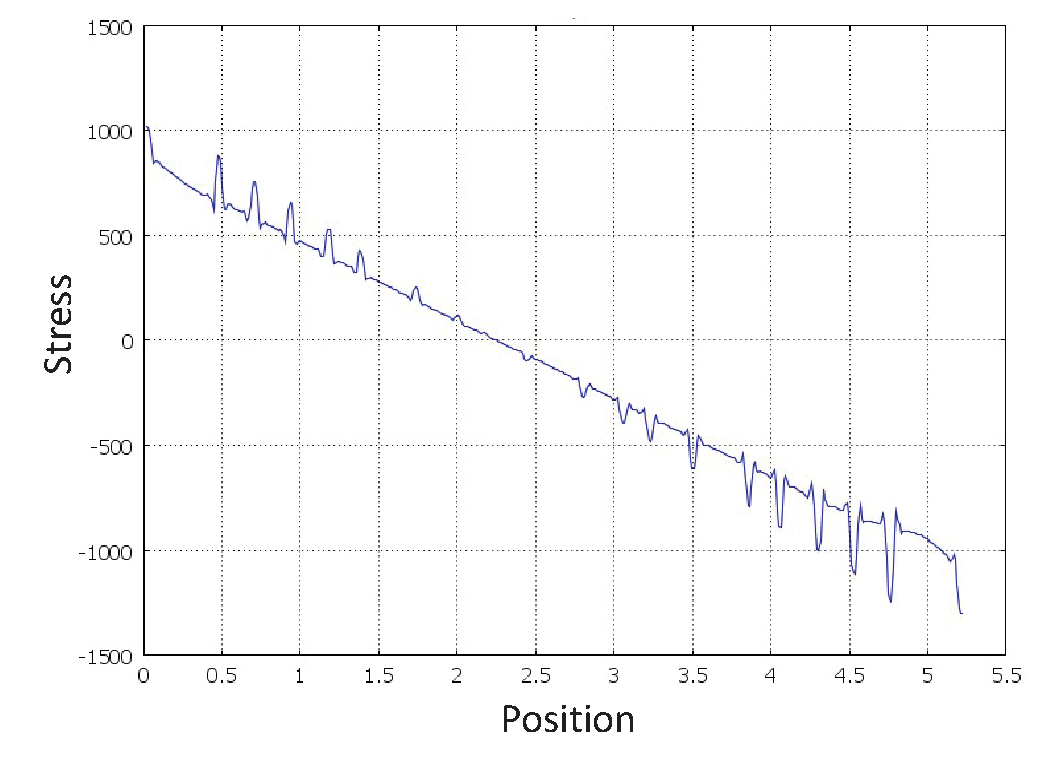
\includegraphics[width=45mm]{3_terminal_stress.eps}
%     \label{fig:3_terminal_stress}}
%     \vspace{-0.04in}
% \caption{(a) Three-terminal interconnect wire; (b) current density distributions; (c) hydrostatic stress distributions. }
%   \label{fig:3_terminal}
%   \vspace{-0.12in}
% \end{figure}

% However, the existing analytical model \eqref{eq:korhonen_sol} focuses
% only on a single segment wire. The research on EM-based stress
% evolutions of both void nucleation and growth phases for multi-segment
% interconnect wires is still a large and challenging problem. Due to
% the strong coupling between neighboring segments, EM reliability of
% multi-segment wires has become a recent major research for being a
% limiting factor in high performance circuit design. To further
% illustrate this, we consider a three-terminal interconnect wire loaded
% with DC currents as shown in Fig. \ref{fig:3_terminal_model}. The
% finite element analysis tool COMSOL \cite{?} can be used to calculate
% the hydrostatic stress along the interconnect wire. The distributions
% of the current density and the hydrostatic stress along this wire are
% shown in Fig. \ref{fig:3_terminal_current} and
% Fig. \ref{fig:3_terminal_stress}, respectively.
%Recent work \cite{?}
% has report an analytical solution of EM-based stress evolution
% equation during the void nucleation phase. But it did not give an
% analytic form to model a general multi-segment interconnect wire. In
% this paper, for the first time, we will propose an analytic method to
% calculate the stress evolution considering EM effects during the void
% nucleation phase for multi-segment interconnect wires.

%The proposed closed-form expression can be used to calculate the hydrostatic stress evolution during the void nucleation phase.





